%* Source (edited from): https://tex.stackexchange.com/a/34303
\documentclass[tikz]{standalone}
\usepackage{pgfplots, calc, tkz-euclide}
\pgfplotsset{compat=1.18}
\usetikzlibrary{decorations.pathreplacing, decorations.markings, angles}
\usepgfplotslibrary{colormaps}
\pgfplotsset{
        colormap/cool,
        % just put all the options in here and it will work as expected
        every axis/.append style={
            axis lines=center,
            tick align=outside,
        },
    }
\begin{document}
% rotated around the x-axis
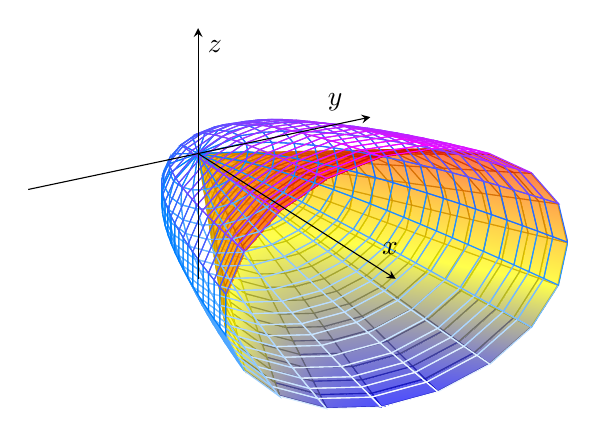
\begin{tikzpicture}
    \def\a{5}
    \def\p{0.1}
    \begin{axis}[view={60}{30},
    ticks=none,
    axis on top,
    xlabel=\(x\), ylabel=\(y\), zlabel=\(z\),]
    \addplot3[surf,
     shader=faceted interp,
     opacity=0.70,
     colormap/hot,
     samples=20,
     domain=0:1,y domain=0:2*pi,
     z buffer=sort]
     (x,{(4.45*x) * cos(deg(y))}, {(4.45*x) * sin(deg(y))});
     \addplot3[mesh,
     samples=20,
     domain=0:1,y domain=0:2*pi,
     z buffer=sort]
     (x,{(2*sqrt(\a*x)) * cos(deg(y))}, {(2*sqrt(\a*x)) * sin(deg(y))});
    \end{axis}
   \end{tikzpicture}
\end{document}